\documentclass[10pt]{exam}
\usepackage[hon]{template-for-exam}
\usepackage{tikz}

\title{A Not-Homework Not-Quiz}
\author{Rohrbach}
\date{\today}

\begin{document}
\maketitle


\noindent
Two positive charges, both of magnitude \SI{5}{\micro\coulomb} sit \SI{0.15}{\meter} away from each other.  Find the net electric field along the $x$-axis at $x=\SI{0.11}{\meter}$.  (\emph{Hint:} $\SI{1}{\micro\coulomb}=\SI{e-6}{\coulomb}$)

\vspace{1em}


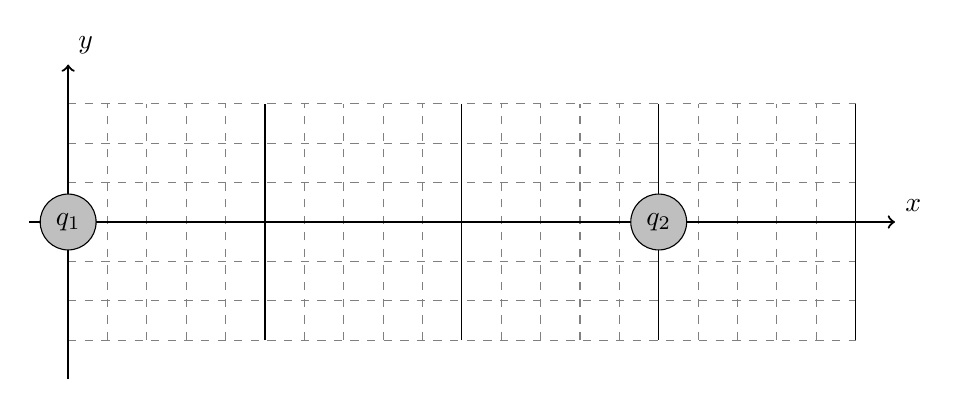
\begin{tikzpicture}[x=0.5cm,y=0.5cm]

  \draw[dashed, thin, gray] (0,-3) grid[step=1] (20,3);
  \draw[black,thin] (0,-3) grid[step=5] (20,3);


  \draw[->,thick] (0,-4) -- (0,4) node[anchor=south west] {$y$};
  \draw[->,thick] (-1,0) -- (21,0) node[anchor=south west] {$x$};


  \node[shape=circle,draw,fill=gray!50] at (0,0) {$q_1$};
  \node[shape=circle,draw,fill=gray!50] at (15,0) {$q_2$};


\end{tikzpicture}

\end{document}